In this section, we will treat a complete example with multiple final products and multiple orders. The goal is to minimize the number of tardy productions. 

\section{Problem statement}

\begin{figure}[h!]
    \centering
    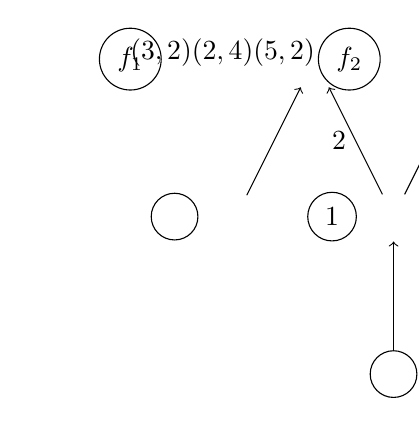
\begin{tikzpicture}
        \draw (0,0) node[circle, draw] (f1) {$f_1$};
        \sopVal{0}{0}{$(3,2)$}
        \draw (2,0) node[circle, draw] (f2) {$f_2$};
        \sopVal{2}{0}{$(2,4)$}
        \draw (-1, -2) node[circle, draw] (RM1) {\vphantom{$f_1$}};
        \draw (1, -2) node[circle, draw] (1) {$1$};
        \sopVal{1}{-2}{$(5,2)$}
        \draw (3, -2) node[circle, draw] (RM2) {\vphantom{$f_1$}};
        \draw (1, -4) node[circle, draw] (RM3) {\vphantom{$f_1$}};

        \draw[->] (RM1) -- (f1);
        \draw[->] (1) -- node[below, left] {$2$} (f1);
        \draw[->] (1) -- (f2);
        \draw[->] (RM2) -- (f2);
        \draw[->] (RM3) -- (1);
    \end{tikzpicture}
    \caption{\label{worked_example:bom}Bill of material}
\end{figure}

The bill of material considered here is represented in figure (\ref{worked_example:bom}). The production system produces two different kinds of final product called "$f_1$" and "$f_2$". Three orders have been made :
\begin{enumerate}
    \item 100 items of product $f_1$
    \item 50 items of product $f_1$ and 100 of product $f_2$
    \item 150 items of product $f_1$ and 50 of product $f_2$
\end{enumerate}

All the orders have been ordered for a given due date $dd = 1200$.

\section{Resolution}

\subsection{First order}

The first order only requires to produce one final product $f_1$. Thus, we can either solve the problem ignoring $f_2$ or enhance the bill of material with a "dummy" product taking into consideration the following mix : \[ mix(f_1) = 1\textrm{ and }mix(f_2) = 0 \]

For the sake of homogeneity, we will do the latter. Let's call $D$ the introduced "dummy product". This choice drives us to the computation of the $n_{iD}$ coefficients. Of course, $n_{f_1D} = 1$ and $n_{f_2D} = 0$ since we only produce $f_1$. We can compute $n_{1D}$ using the general formula, summing the required amount of items to be produced in every path to $D$ starting from item $1$. Since the path going through $f_2$ is valuated as $0$, the following holds :
\[ n_{1D} = n_{1f_1}n_{f_1D} + n_{1f_2}n_{f_2D} = 2.1 + 0.1 = 2 \]

The maximum production rate is computed in the same way as we did (note however that the dummy machine "D" must not be taken into account since it has $0$ setup time and $0$ operational time and can be regarded as a trick to generalize our model to the multiple final product situation.) :
\[
    \begin{split}
        X_f^{max} &= \max_i\left( \frac{b_D}{T_{si} + T_{oi}b_{D}n_{iD}} \right) \\
        &= \max\left(
            \underbrace{\frac{b_D}{3+2.b_D.1}}_{f_1} ; 
            \underbrace{\frac{b_D}{2+4.b_D.0}}_{f_2} ; 
            \underbrace{\frac{b_D}{5+2.b_D.1}}_{1}
        \right)
    \end{split}
\]
A very brief analysis of this function of $b_f$ should yield that machine $1$ will always be the bottleneck machine, independtly of $b_f$ (which is not the general case) since the y-intercept and slope of the denominators is higher for machine $1$ than any of the two other machines.

Thus, we can be confident about using the formula giving the optimal batch size given the bottleneck machine. This yields : 
\[
    b_D^\circ= \sqrt{ \frac{100.5}{(2-1).2.2}} \approx 11
\]
One important thing to be noted however is how the length $L$ of the bom of material has been computed \textit{without} taking into account the dummy product. In fact, and this will become even clearer when we will compute the production time. The formula derives (literally) from the approximation that the first bacth of final product can be produced after a time of $L.D$. But since the "dummy" product is not "manufactured" in reality (in the sense that we have no setup time nor operational time), we shall not count another production cycle for it to be made. Hence the consideration that $L = 2$. 

Regarding the production time indeed, it can be computed as follow : 
\[
    \begin{split}
        T_{prod}(100f_1)|_{b_D = 11} &= \left(2-1+\left\lceil \frac{100}{11} \right\rceil\right)T_b(11) \\
        &= 11\times(5+2.11.2) = 539
    \end{split}
\]

\subsection{Second order}

Concerning the second order, we have now to deal with a "real" multiple final product order. The mix of production can be regarded as the percentage of one final product over the whole production. Hence, 
\[
    mix(f_1) = \frac{50}{50 + 100} = \frac{1}{3}\textrm{ and }
    mix(f_2) = \frac{100}{50 + 100} = \frac{2}{3}
\]
It becomes clear that the best choice for $n_{f_1D}$ and $n_{f_2D}$ is, respectively, $1$ and $2$, obtained by multiplying the mixes of production by $3$. Thus, the number of items $1$ needed to produced one item $D$ becomes \[ n_{1D} = n_{1f_1}n_{f_1D} + n_{1f_2}n_{f_2D} = 2.1+1.2 = 4 \]

The same computations as before can be done to compute the maximum production rate which yields the following : 
\[ X_f^{max} = \max\left( \frac{b_D}{3+2b_D} ; \frac{b_D}{2+8b_D} ; \frac{b_D}{5+8b_D} \right) \]
which again, and for the same reasons, gives us the same bottleneck machine (machine $1$). 

The optimal batch sizing for that order now becomes $b_D^\circ = \sqrt{ \frac{150.5}{(2-1).2.4} }\approx 10$ and the production time for that order is comuted as 
\[ T_{prod}(50f_1 + 100f_2)|_{b_D = 10} = \left( 2-1+\left\lceil \frac{150}{10} \right\rceil \right)T_b(10) = 16\times(5+2.10.4) = 1360 \]

\subsection{Third order}

Finally, the last order can be treated using the following production mix :
\[ mix(f_1) = \frac{150}{200} = \frac{3}{4} \textrm{ and } mix(f_2) = \frac{50}{200} = \frac{1}{4} \] which yields the following coefficients : \[ n_{f_1D} = 3\textrm{ ; }n_{f_2D} = 1\textrm{ ; }n_{1D} = 3.2 + 1.1 = 7 \]
(the first two coefficients being obtained by multiplying the production mixes by $4$). 

Again, computing the maximum production rate will yield machine $1$ as the bottleneck machine independently of the batch size used. And the optimal batch size is given by the same computations $b_D^\circ = \sqrt{ \frac{200.5}{(2-1).2.7} } = 8$. Using such a batch size, the production time is simply given by 
\[
    T_{prod}(150f_1 + 50f_2)|_{b_D = 8} = \left(2-1+\left\lceil \frac{200}{8} \right\rceil\right)T_b(8)
    = 26\times(5+2.8.7) = 3042
\]

\subsection{Production scheduling}

The results previously obtained are sumed up as the following, where $T_{O_i}$ denotes the production time of the $i$th order :
\[
    \begin{split}
        T_{O_1} &= 539\\
        T_{O_2} &= 1360\\
        T_{O_3} &= 3042
    \end{split}
\]
The due date of each order was $1200$ while the overall makespan can be computed as \[ \sum_i T_{O_i} = 4941 \]
It is clear that not all the tasks can be fulfilled before their respective due date. In fact, it seems obvious that the only task which can be early or at most jsut in time is the first order. The two other tasks will be tardy, irreverently of their order. Thus the production schedule should be the following :
\begin{center}
    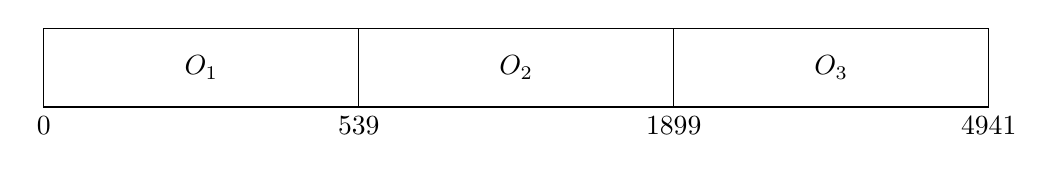
\begin{tikzpicture}[xscale=4]
        \draw (0,0) node[below] {$0$} rectangle node {$O_1$} (1, 1);
        \draw (1,0) node[below] {$539$} rectangle node {$O_2$} (2, 1);
        \draw (2,0) node[below] {$1899$} rectangle node {$O_3$} (3, 1);
        \draw (3,0) node[below] {$4941$};
    \end{tikzpicture}
\end{center}